%\documentclass[]{spie}  %>>> use for US letter paper
\documentclass[a4paper]{spie}  %>>> use this instead for A4 paper
%\documentclass[nocompress]{spie}  %>>> to avoid compression of citations

\renewcommand{\baselinestretch}{1.0} % Change to 1.65 for double spacing
 
\usepackage{amsmath,amsfonts,amssymb}
\makeatletter
\let\jnl@style=\rmfamily
\def\ref@jnl#1{{\jnl@style#1}}%
\newcommand\aap{\ref@jnl{A\&A}}%
\usepackage{graphicx}
\usepackage[colorlinks=true, allcolors=blue]{hyperref}
 \usepackage{multirow}
\title{A Kanban approach for the Sardinia Radio Telescope operations}

\author[a]{Sergio Poppi}
\author[a]{Emilio Molinari}
\affil[a]{INAF Osservatorio Astronomico di Cagliari, Via della Scienza 5, Selargius (CA) , Italy}
 
\authorinfo{Further author information: (Send correspondence to Sergio Poppi)\\ E-mail: sergio.poppi@inaf.it, Telephone:+39 07071180265 \\}

% Option to view page numbers
\pagestyle{empty} % change to \pagestyle{plain} for page numbers   
\setcounter{page}{301} % Set start page numbering at e.g. 301
 
\begin{document} 
\maketitle

\begin{abstract}
The Sardinia Radio Telescope,SRT,  is a 64-metre  radio telescope  operated by the  National Institute for Astrophysics (INAF). It is a general purpose instrument  with frequency agility and wide frequency coverage. 
Operations can be represented as a continuous flow of actions that must be taken in charge by the team, with the goal to minimize  the downtime an maximize the scientific outcome of the facility. Also, operating partly in guest mode, the overall satisfaction of the observers is a goal to be achieved.
Following  the of Agile principles derived from software development, we intend to implement a  Kanban approach. Hence, we will identify internal sectors as a series of  manifolds  of client-producer chain, and monitor the workflow with kanban-like tickets. An electronic version of Kanban will enable coordinators  to have an at-a-glance view of the critical points.
\end{abstract}

% Include a list of keywords after the abstract 
\keywords{Radiotelescope, operations, Kanban}

\section{INTRODUCTION}
\label{sec:intro}  % \label{} allows reference to this section



The Sardinia Radio Telescope is an observing facility managed by the Istituto Nazionale di Astrofisica (\href{http://www.inaf.it}{INAF}).  
It is a 64-metre radio telescope, designed to operate  at  frequencies ranging from 300 Mhz to 116 GHz  [\cite{2015JAI.....450008B}].
It is a versatile telescope, covering a wide range of frequency, with a high agility of receiver switching. This  allows the telescope to be suitable for many scientific topic like pulsars, interstellar medium, astrochemistry, space weather[\cite{prandoni}].

For 80\% of the time, SRT is operated by INAF, for  the remaining 20\% by Agenzia Spaziale Italiana (\href{http://www.asi.it}{ASI})  for probe tracking and deep space  activities. 
Furthermore, SRT is part of  to the European Vlbi Network (\href{https://www.evlbi.org/}{EVN}), a network of telescope operating in Very-long baseline interferometric mode.

Time allocation is summarized as follows:
\begin{itemize}
    \item Europenan VLBI Network time (~25\%)
    \item Time allocated by INAF for Single-dish observations (~40\%)
    \item Director's discretionary time (5\%)
    \item Maintenance (10\%)
    \item ASI time(20\%)
\end{itemize}

Observations are run mainly guest mode, where observers are asked to operate on site. However, for the 20\% of the running time it operates in service mode 
Users who require for observing time submit an observing proposal during call for proposal which are published twice a year. Then proposal are evaluated by the time-allocation-committee and then if accepted, set to the scheduler who has in charge the time allocation task. 

To run an observing facility many aspects have to be taken into account. In the following sections we describe how operations are are organized. 

\begin{figure} [hbt!]
   \begin{center}
   \begin{tabular}{c} 
   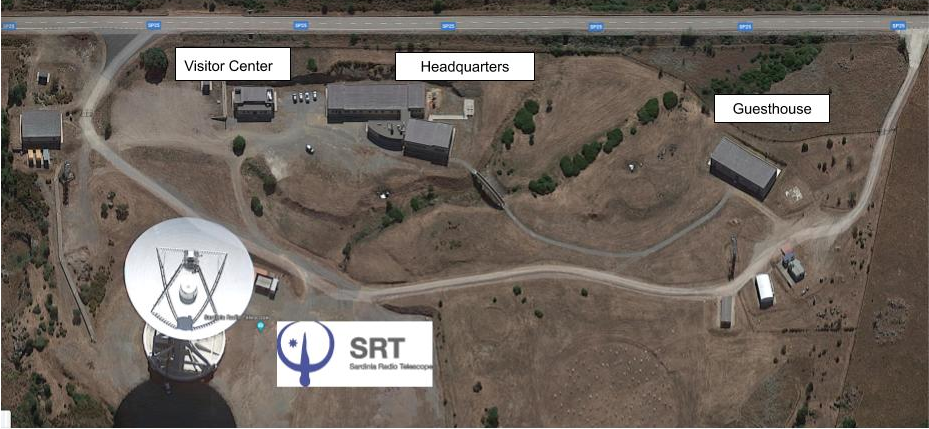
\includegraphics[width=1.0\textwidth]{srt_site.png}
	\end{tabular}
	\end{center}
   \caption[example] 
   { \label{fig:srt_site} 
The SRT area covers about 140 000 m$^2$ and includes headquarters, a guesthouse, a visitor center and the telescope.  }.
   \end{figure} 

\section{Operations}
Day to day operations are made of a continuous stack of actions which are mandatory  to maximize the effective time of the telescope and the support to the observers. Being an observing facility, all the activity concerning operations  are run to maximize the effective up-time of the telescope and its functionality at its best performances.
SRT Operations are run by the operating team. The coordinator is the Head of Operations, who as the role of Operation Manager. 
Activities are divided in 10 Macro Work Packages which are organized in one or more packages:
Table~\ref{tab:team_strutture} summarizes the structure of the team. 

\begin{table}[hbt!]
    \centering
    \begin{tabular}{|l |l|}
    \hline
\rule[-1ex]{0pt}{3.5ex}    \textbf{ Macro Work Package}     & \rule[-1ex]{0pt}{3.5ex} \textbf{Work Package}     \\ 
   \hline
    \hline

\rule[-1ex]{0pt}{3.5ex}    \multirow{1}{*}{Receivers, Down-conversion,IF \& Feeds}       & \rule[-1ex]{0pt}{3.5ex} Receivers operativity     \\ 
   \hline
\rule[-1ex]{0pt}{3.5ex}     \multirow{4}{*}{Metrology}                                   & \rule[-1ex]{0pt}{3.5ex}  Metrology and optics\\
                                                                 &  \rule[-1ex]{0pt}{3.5ex} RFI Monitoring \\     
                                                                 &  \rule[-1ex]{0pt}{3.5ex} Time \& Frequency \\   
                                                                 & \rule[-1ex]{0pt}{3.5ex} Weather \& GPS \\
\hline                                                
\rule[-1ex]{0pt}{3.5ex}      \multirow{1}{*}{Backends and VLBI terminals}                & \rule[-1ex]{0pt}{3.5ex} HW \& SW backends functionality \\
\hline
\rule[-1ex]{0pt}{3.5ex}      \multirow{2}{*}{ICT Department}                            & \rule[-1ex]{0pt}{3.5ex} Scientific Services \\
                                                                                        & \rule[-1ex]{0pt}{3.5ex} General Services  \\
\hline
\rule[-1ex]{0pt}{3.5ex}      \multirow{5}{*}{Users support}                             & \rule[-1ex]{0pt}{3.5ex}  Observation optimization \\
                                                                                        & \rule[-1ex]{0pt}{3.5ex} Documentation \\
                                                                                        & \rule[-1ex]{0pt}{3.5ex} Users support and training \\
                                                                                        & \rule[-1ex]{0pt}{3.5ex} Scientific Software support \\
                                                                                        & \rule[-1ex]{0pt}{3.5ex} VLBI Operations \\
\hline
\rule[-1ex]{0pt}{3.5ex}      \multirow{1}{*}{Outreach}                                  & \rule[-1ex]{0pt}{3.5ex}  Outreach and visitors management \\
\hline 
\rule[-1ex]{0pt}{3.5ex}      \multirow{4}{*}{Site Management, Plants, telescope servo systems} & \rule[-1ex]{0pt}{3.5ex}  Infrastructure, plants, logistic \\
                                                                                        & \rule[-1ex]{0pt}{3.5ex} Servo systems and telescope plants \\
                                                                                        & \rule[-1ex]{0pt}{3.5ex} Contracts management\\
                                                                                        &\rule[-1ex]{0pt}{3.5ex}  Visitors services \\
\hline 
\rule[-1ex]{0pt}{3.5ex}     \multirow{1}{*}{Telescope Mechanics}                         & \rule[-1ex]{0pt}{3.5ex} Telescope,Receivers and Servo systems mechanics \\
\hline
\rule[-1ex]{0pt}{3.5ex}     \multirow{1}{*}{Safety management}                          & \rule[-1ex]{0pt}{3.5ex} Workers Safety \\
\hline
\rule[-1ex]{0pt}{3.5ex}     \multirow{1}{*}{Interface with ASI Operations}               & \rule[-1ex]{0pt}{3.5ex} Interface with ASI \\
\hline
    \end{tabular}
    \caption{Operating Team is  organized in macro  work packages and work packages}
    \label{tab:team_strutture}
\end{table}

  \begin{figure} [!hb]
   \begin{center}
   \begin{tabular}{c} 
   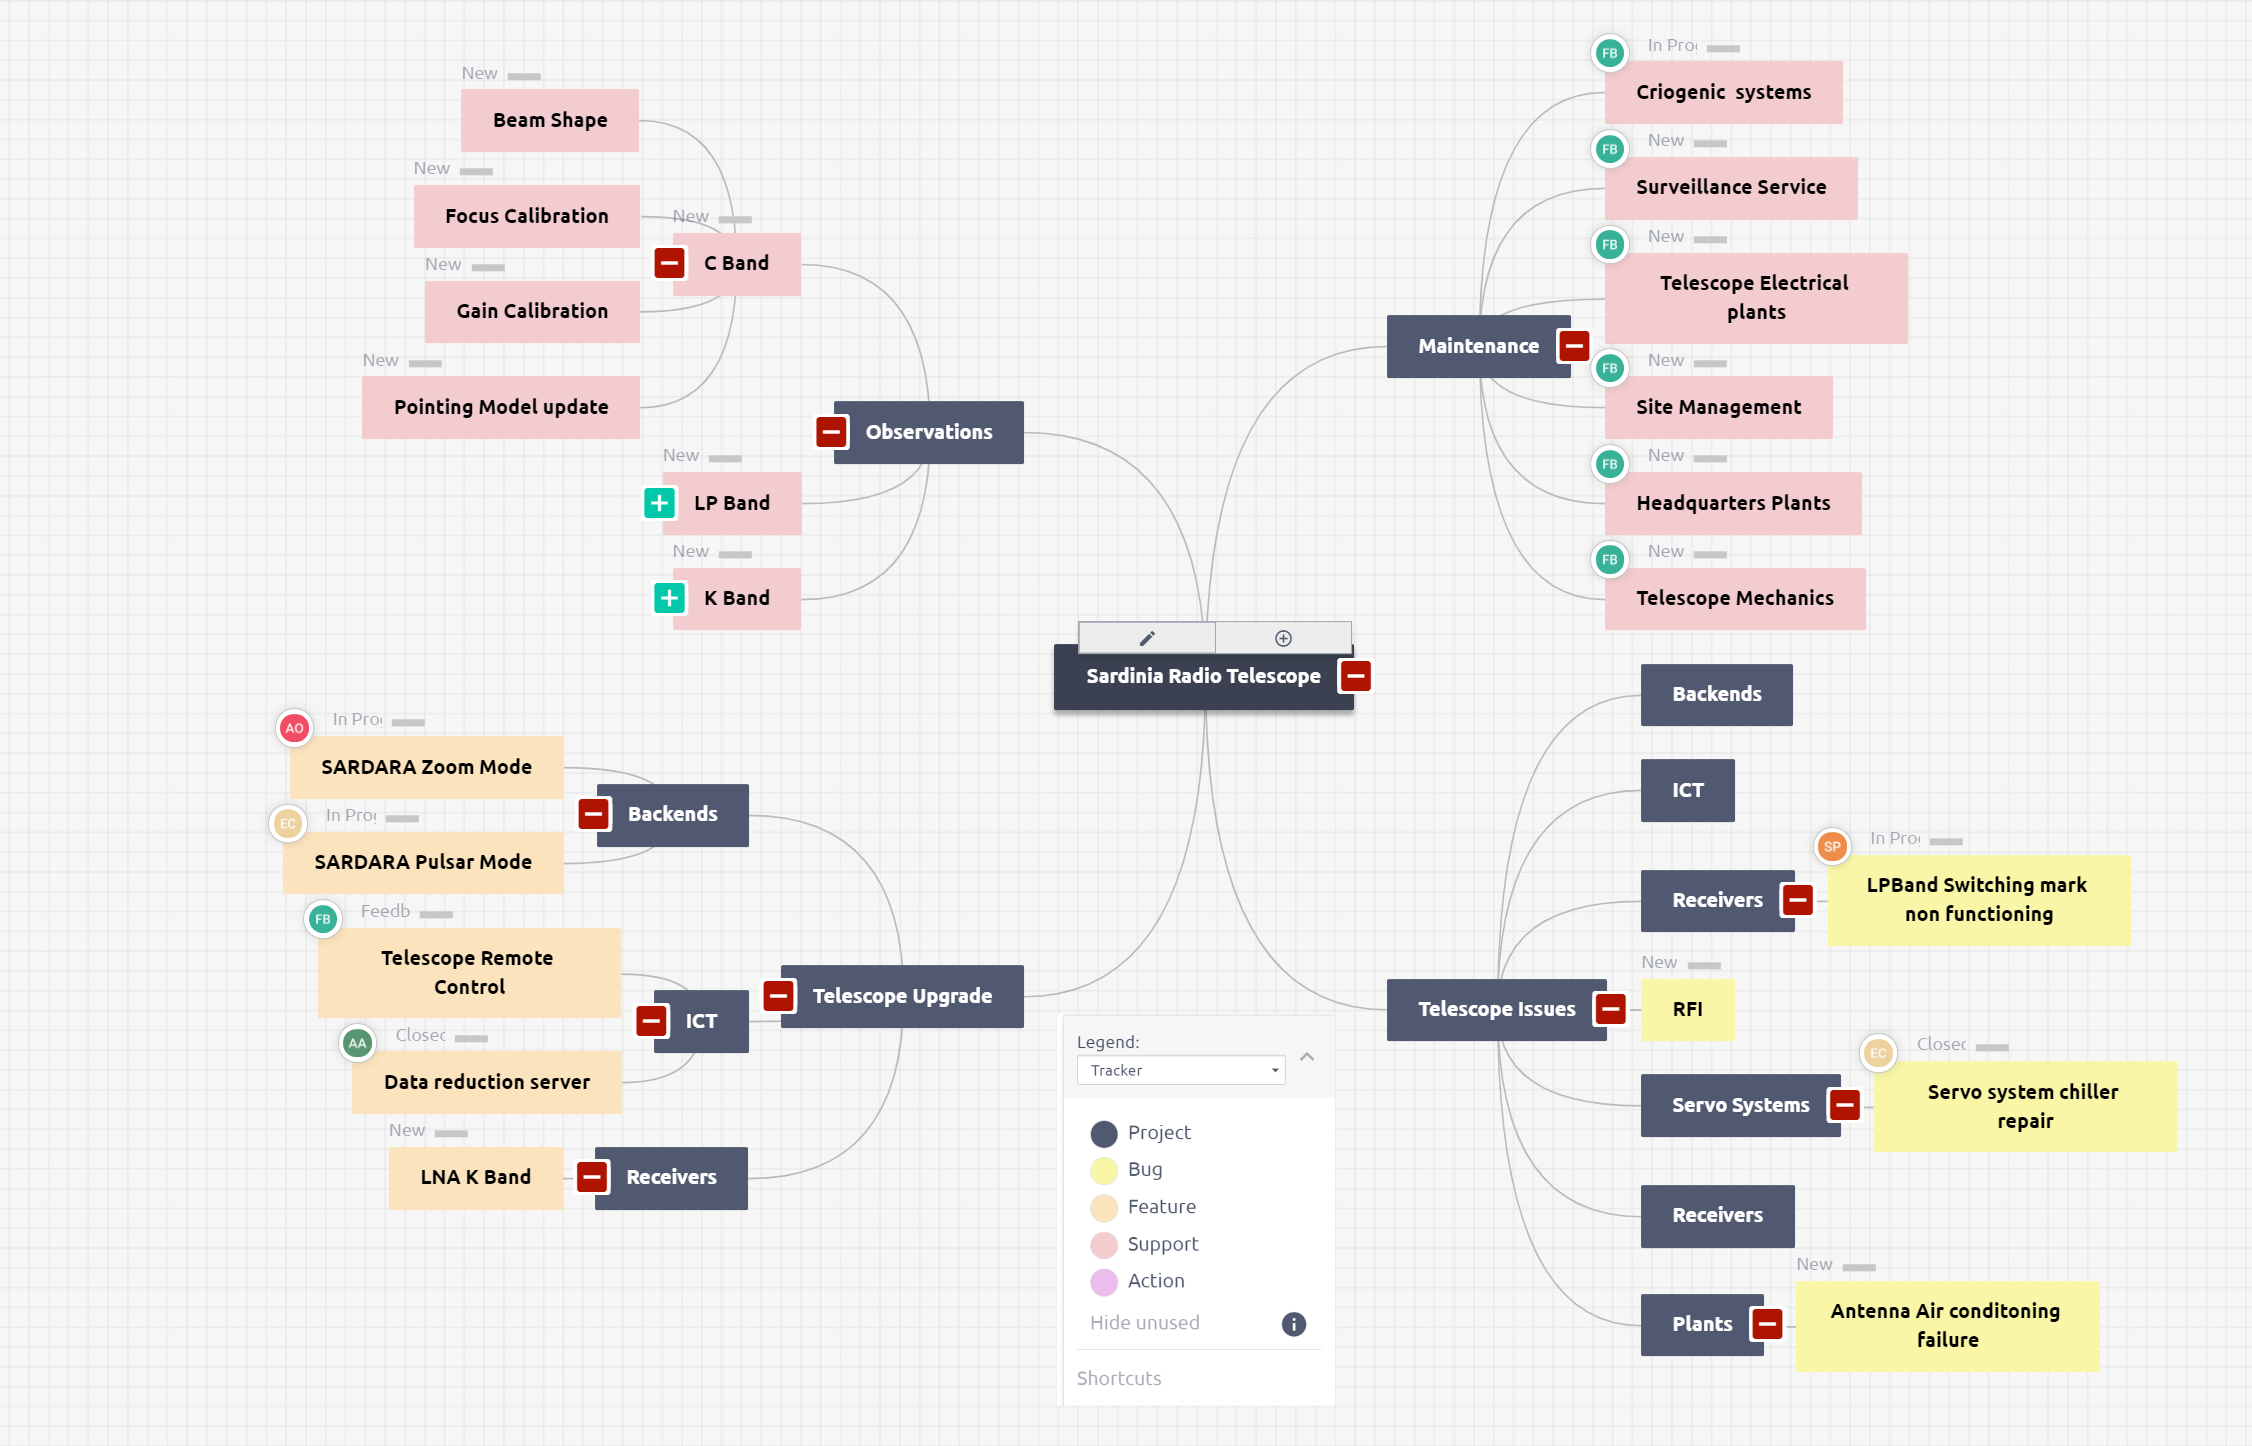
\includegraphics[width=\textwidth]{detailed_wbs.png}
	\end{tabular}
	\end{center}
   \caption[example] 
   { \label{fig:wbs} Operations are grouped in maintenance, telescope issues, telescope upgrades and support to observations. Issues can refer to bugs, new features or supporting atcivities.}

   \end{figure} 
Operations are grouped in maintenance, telescope issues, telescope upgrades and support to observations. The structure is outlined in Figure~\ref{fig:wbs}. 

Maintenance applies to the telescope with its electrical plants, cryogenics systems and structure, to the  headquarters and to the whole SRT area. Maintenance activities are  outsourced with 
a \textit{contract director} belonging to the operating team who has in charge the supervision of the contract.   
Antenna Maintenance follows a working plan which defines activities and their periodicity. 
%Operativity requires thus a a continuous flow of actions that involves many topics.  

Telescope issues include fault report and bugs which could occur while the telescope is observing or any other malfunctioning that could prevent the regular working. 

Beside this, telescope upgrade groups the task for improving the functionalities of the telescope, like observing modes, new hardware or software improvement.


Observations support starts just after a project is approved. First,  the telescope scheduler allocates the needed time slot for each telescope. Then, the User Support team contact the PI of each experiment to fix details of the forthcoming observations, and a project friends is assigned to support the proposers in the experiment setup. 

\section{An Agile methodology: Kanban }
Kanban has origins from Toyota Production System (TPS) which is based on two pillars, the just-in-time production and autonomation. 
These  concepts allow the implementation of a production system which is optimized in terms of sustainability, delivering only what is needed, 
in the time that is needed.
The other pillar is  the autonomation:  automation with human touch \cite{tps}. 

\textit{Kanban} is one of the operational items of the TPS. Litterally, {\it kanban} means {\it cards}, which could represent  a piece of work. the production process is visualized  on a board where each stage of the process is represented. Moving the cards along each stage the flow of the process can be easily followed. 
Usually, cards start from a {\it to do area}, crossing intermediate steps, getting to  {\it done}.
\begin{figure} [ht]
   \begin{center}
   \begin{tabular}{c} 
   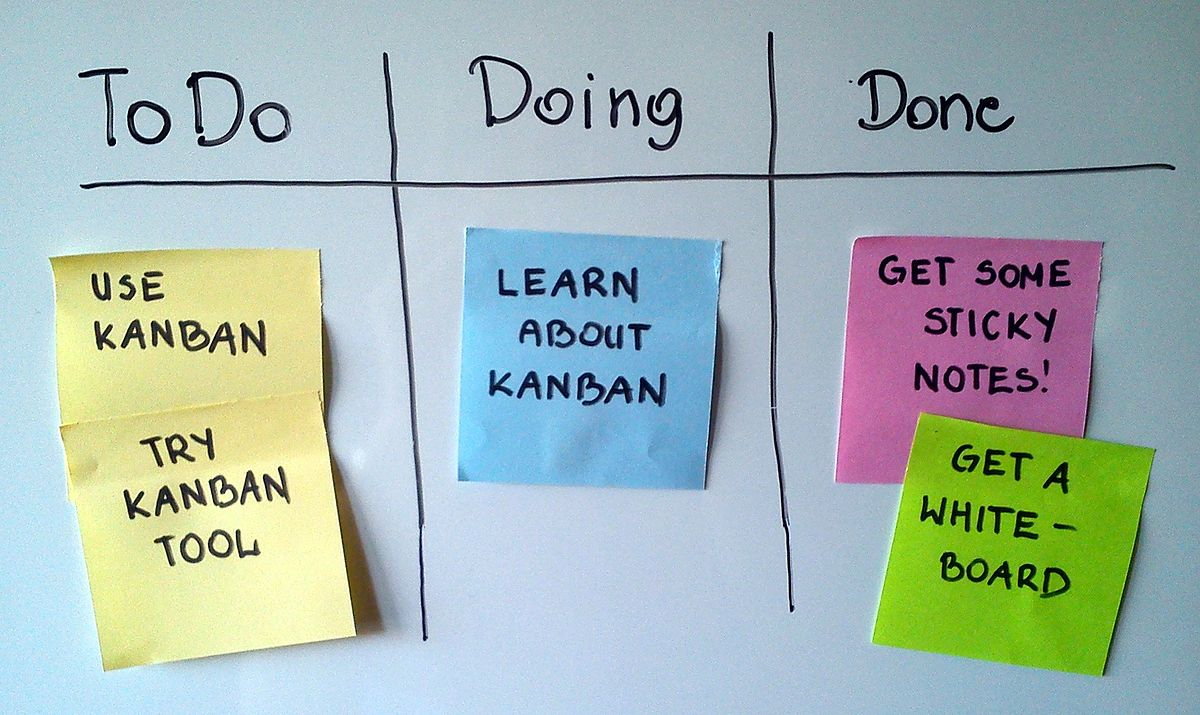
\includegraphics[width=0.5\textwidth]{1200px-Simple-kanban-board-.jpg}
	\end{tabular}
	\end{center}
   \caption[example] 
   { \label{fig:kanban} Example of a simple kanban board (picture  by  \href{https://commons.wikimedia.org/wiki/File:Simple-kanban-board-.jpg}{Jeff Lasovski)}
 }.
   \end{figure} 
 Only a limited number of cards can be put on the board. This puts a limit on the possible work in progress, allowing a news {\it to-do} card, only
 after another card get {done}, meaning that the task is done. In this way, the work in progress is limited, allowing only what is sustainable to proceed along the production line.
 Kanband  started with production processes, however, since then it has been applied to other fields in project management  like software development\cite{brech15}. 
Applied to software development, Kanban methodology follows the principles stated in the manifesto for Agile Software Development
\footnote{http://agilemanifesto.org}   Generally,  Kanban is built for smooth and continuous delivery of customer value \cite{brech15}.


\section{Kanban at SRT}



\begin{figure} [!ht]
   \begin{center}
   \begin{tabular}{c} 
   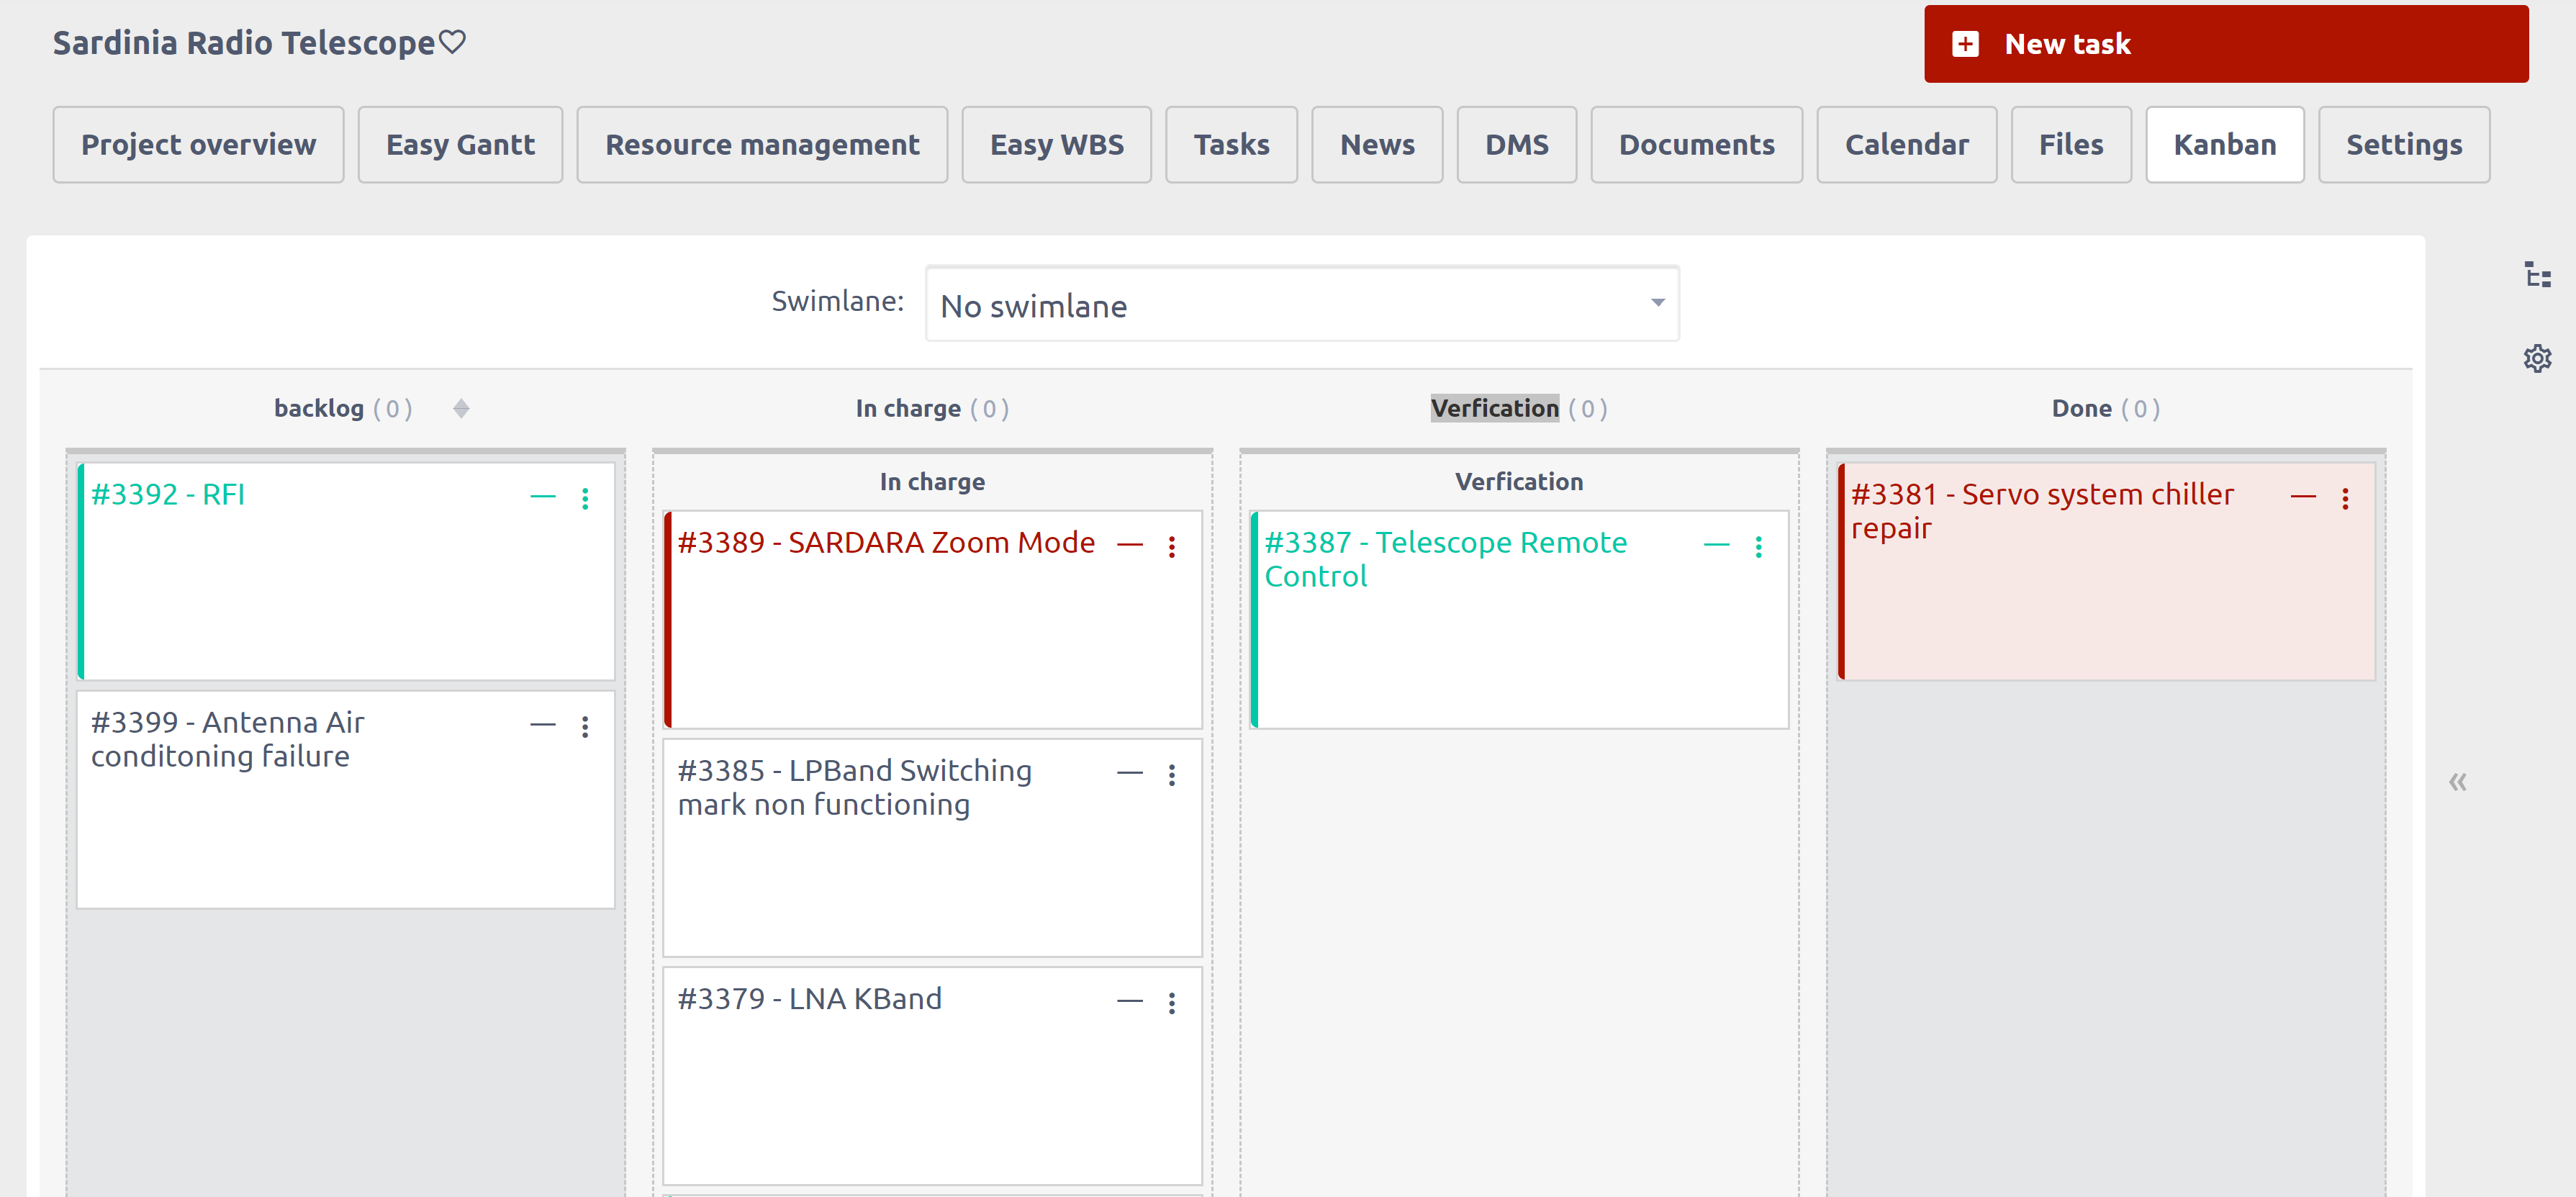
\includegraphics[width=0.9\textwidth]{kanbanboard.png}
	\end{tabular}
	\end{center}
   \caption[example] 
   { \label{fig:kanbansrt} SRT Operations Kanban  board. Cards flow from the leftmost column towards the \textit{done} one, when the issue is closed. Each cards contains tracking information, like due date, priority, and assignee.}

   \end{figure} 

There are two kind of issues that an operation manager has to deal with. First, there are issues which can be planned  in advance, like for example  maintenance periodicity and contracts. 
Other issues can not be foreseen, like malfunctioning, failures, or bugs.

Information concerning unpredictable issues could come from several sources: from a ticketing system opened by observers, sent by email or through the feedback form that observers are asked to fill.
The operation manager has to check that all kind of issues are tracked and put to the attention of the operating team. 
A project management software can help track the issue. To do this, we have been using Easy Redmine a commercial implementation of open source Redmine\footnote{\url{https://www.redmine.org/}}.  

For each issue,  a \textit{task} is created with attributes defining  priority, due date and a possible assignment.
The Operation Manager inserts the task in the backlog. The backlog is the first column of the SRT  Kanban board which is  showed in Figure~\ref{fig:kanbansrt}. The other three columns are  \textit{in charge}, \textit{verification}, \textit{closed}.

The backlog represents the\textit{ to-do list}. The card representing the task can give information about the priority, due date and assignment.
The backlog can be sorted by priority. In Figure~\ref{fig:kanbansrt} is the left most column. The Operations Manager assigns the task and when the assignee starts the work, moves the card to the right, in the {in charge} column. Once the task is supposed to be completed, the assignee moves the card to \textit{verification}, where the issue is tested to verify if it is really  solved. If the issue is  related to a telescope failure, the role to check the verification is passed is in charge to the User Support, who has among his duties to assure the  telescope is at its performances. Otherwise, is the \textit{Site Manager} who leads the Site Management Macro Working Package to check the verification process is completed. At this point, the card is moved to \textit{done}, the rightmost column. 

After completion of the verification process, the card gets to the rightmost column. 
This means that the process is  \textit{done} and the issue can be \textit{closed}.

This is nearly the beginning of Kanban at SRT, in the next phase we will collect statistics about timings of the various phase, so that it will be possible to track the most used areas, the least staffed work packages and try to reduce downtime by reallocating resources.



\section{Conclusions}

With respect traditional waterfall tracking issues methods, Kanban improves the efficiency of running operations.
From one hand, the Kanban board helps the manager and the team  visualize the flow of the process, concerning the issues. It can be possible to view at which stage is set each task, highlighting the bottlenecks.

On the other side, limiting the number of allowed cards, the work in progress is also limited because the team takes in charge only the tasks that  can be afforded.
 
\acknowledgments % equivalent to \section*{ACKNOWLEDGMENTS}       


 
The Sardinia Radio Telescope is funded by the Ministry of University and Research (MIUR), Italian Space Agency (ASI), and the Autonomous Region of Sardinia (RAS) and is operated as National Facility by the National Institute for Astrophysics (INAF)

% References
\bibliography{report} % bibliography data in report.bib
\bibliographystyle{spiebib} % makes bibtex use spiebib.bst

\end{document} 
